
\documentclass[11pt,letterpaper]{article}

\usepackage[utf8]{inputenc}
\usepackage[T1]{fontenc}
\usepackage{lmodern}
\usepackage{amsmath,amssymb,amsfonts,amsthm}
\usepackage{mathtools}
\usepackage{bm}
\usepackage{graphicx}
\graphicspath{{Graphics/}}
\usepackage{float}
\usepackage{subcaption}
\usepackage{booktabs}
\usepackage[margin=0.85in]{geometry}
\usepackage{microtype}
\usepackage{enumitem}
\usepackage{titlesec}
\usepackage[hidelinks]{hyperref}

\setlength{\parindent}{0pt}
\setlength{\parskip}{5pt}

\titlespacing*{\section}{0pt}{10pt}{4pt}
\titlespacing*{\subsection}{0pt}{7pt}{3pt}

\newcommand{\R}{\mathbb{R}}
\newcommand{\norm}[1]{\left\lVert #1 \right\rVert}
\newcommand{\grad}{\nabla}
\newcommand{\lap}{\Delta}
\newcommand{\uvec}{\bm{u}}

\title{\vspace{-1.5cm}
    \textbf{Immersed Boundaries}\\
    \large Poisson Equation with Immersed Boundary
}
\author{Luciano Henriquez}
\date{}

\begin{document}

\maketitle
\vspace{-0.6cm}

% --------------------------------------------------
\section{Introduction}
% --------------------------------------------------

We consider the Poisson equation on the domain $\Omega  = (0,2\pi )^2$
\begin{equation}
    \begin{aligned}
        \grad ^2u &= f(x,y), \quad (x,y)\in (0,2\pi )^2 \\
    \end{aligned}
  \end{equation}
subject to Dirichlet boundary conditions, before ultimately proceeding to the Poisson equation with an immersed boundary. We commence by solving eq 1 by discretizing the square grid using the five point Laplacian finite difference approximation. We verify the validity of our approximation using the method of manufactured solutions, where the test solution is $u(x,y) = \cos 2x \sin 2y$, so that $f(x,y) =-8\cos 2x \sin 2y $.
% --------------------------------------------------
\section{Simple Poisson Equation}
% --------------------------------------------------

As discussed above, using the method of manufactured solutions and using matlab we get the following plots:

\begin{figure}[H]
    \centering
    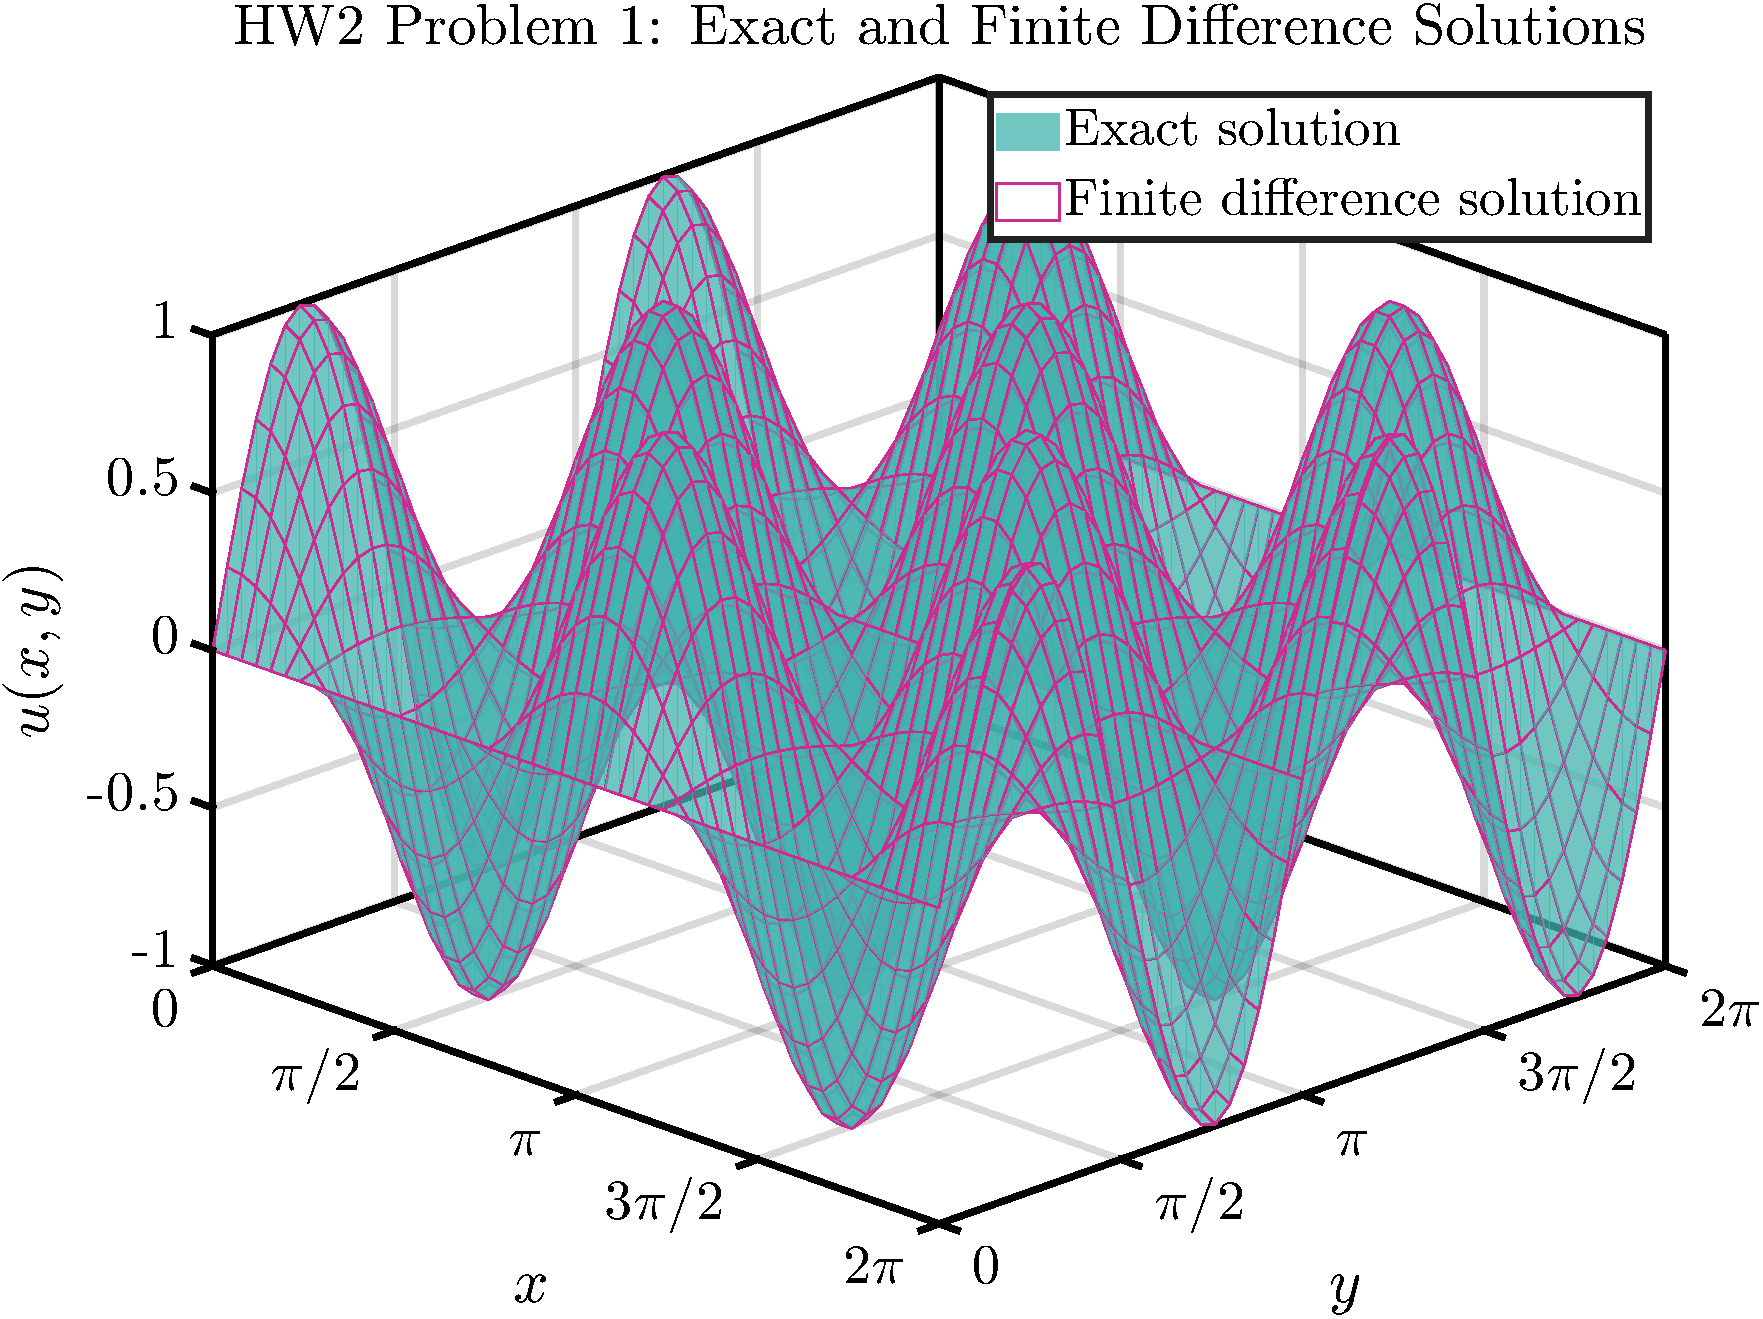
\includegraphics[width=0.70\linewidth]{poisson_hw2_problem1_solution.pdf}
    \caption{Exact solution $u(x,y)=\cos 2x \sin 2y$ (shaded surface) and the approximate solution (purple mesh)}
    \label{fig:poisson-solution}
\end{figure}

\begin{figure}[H]
    \centering
    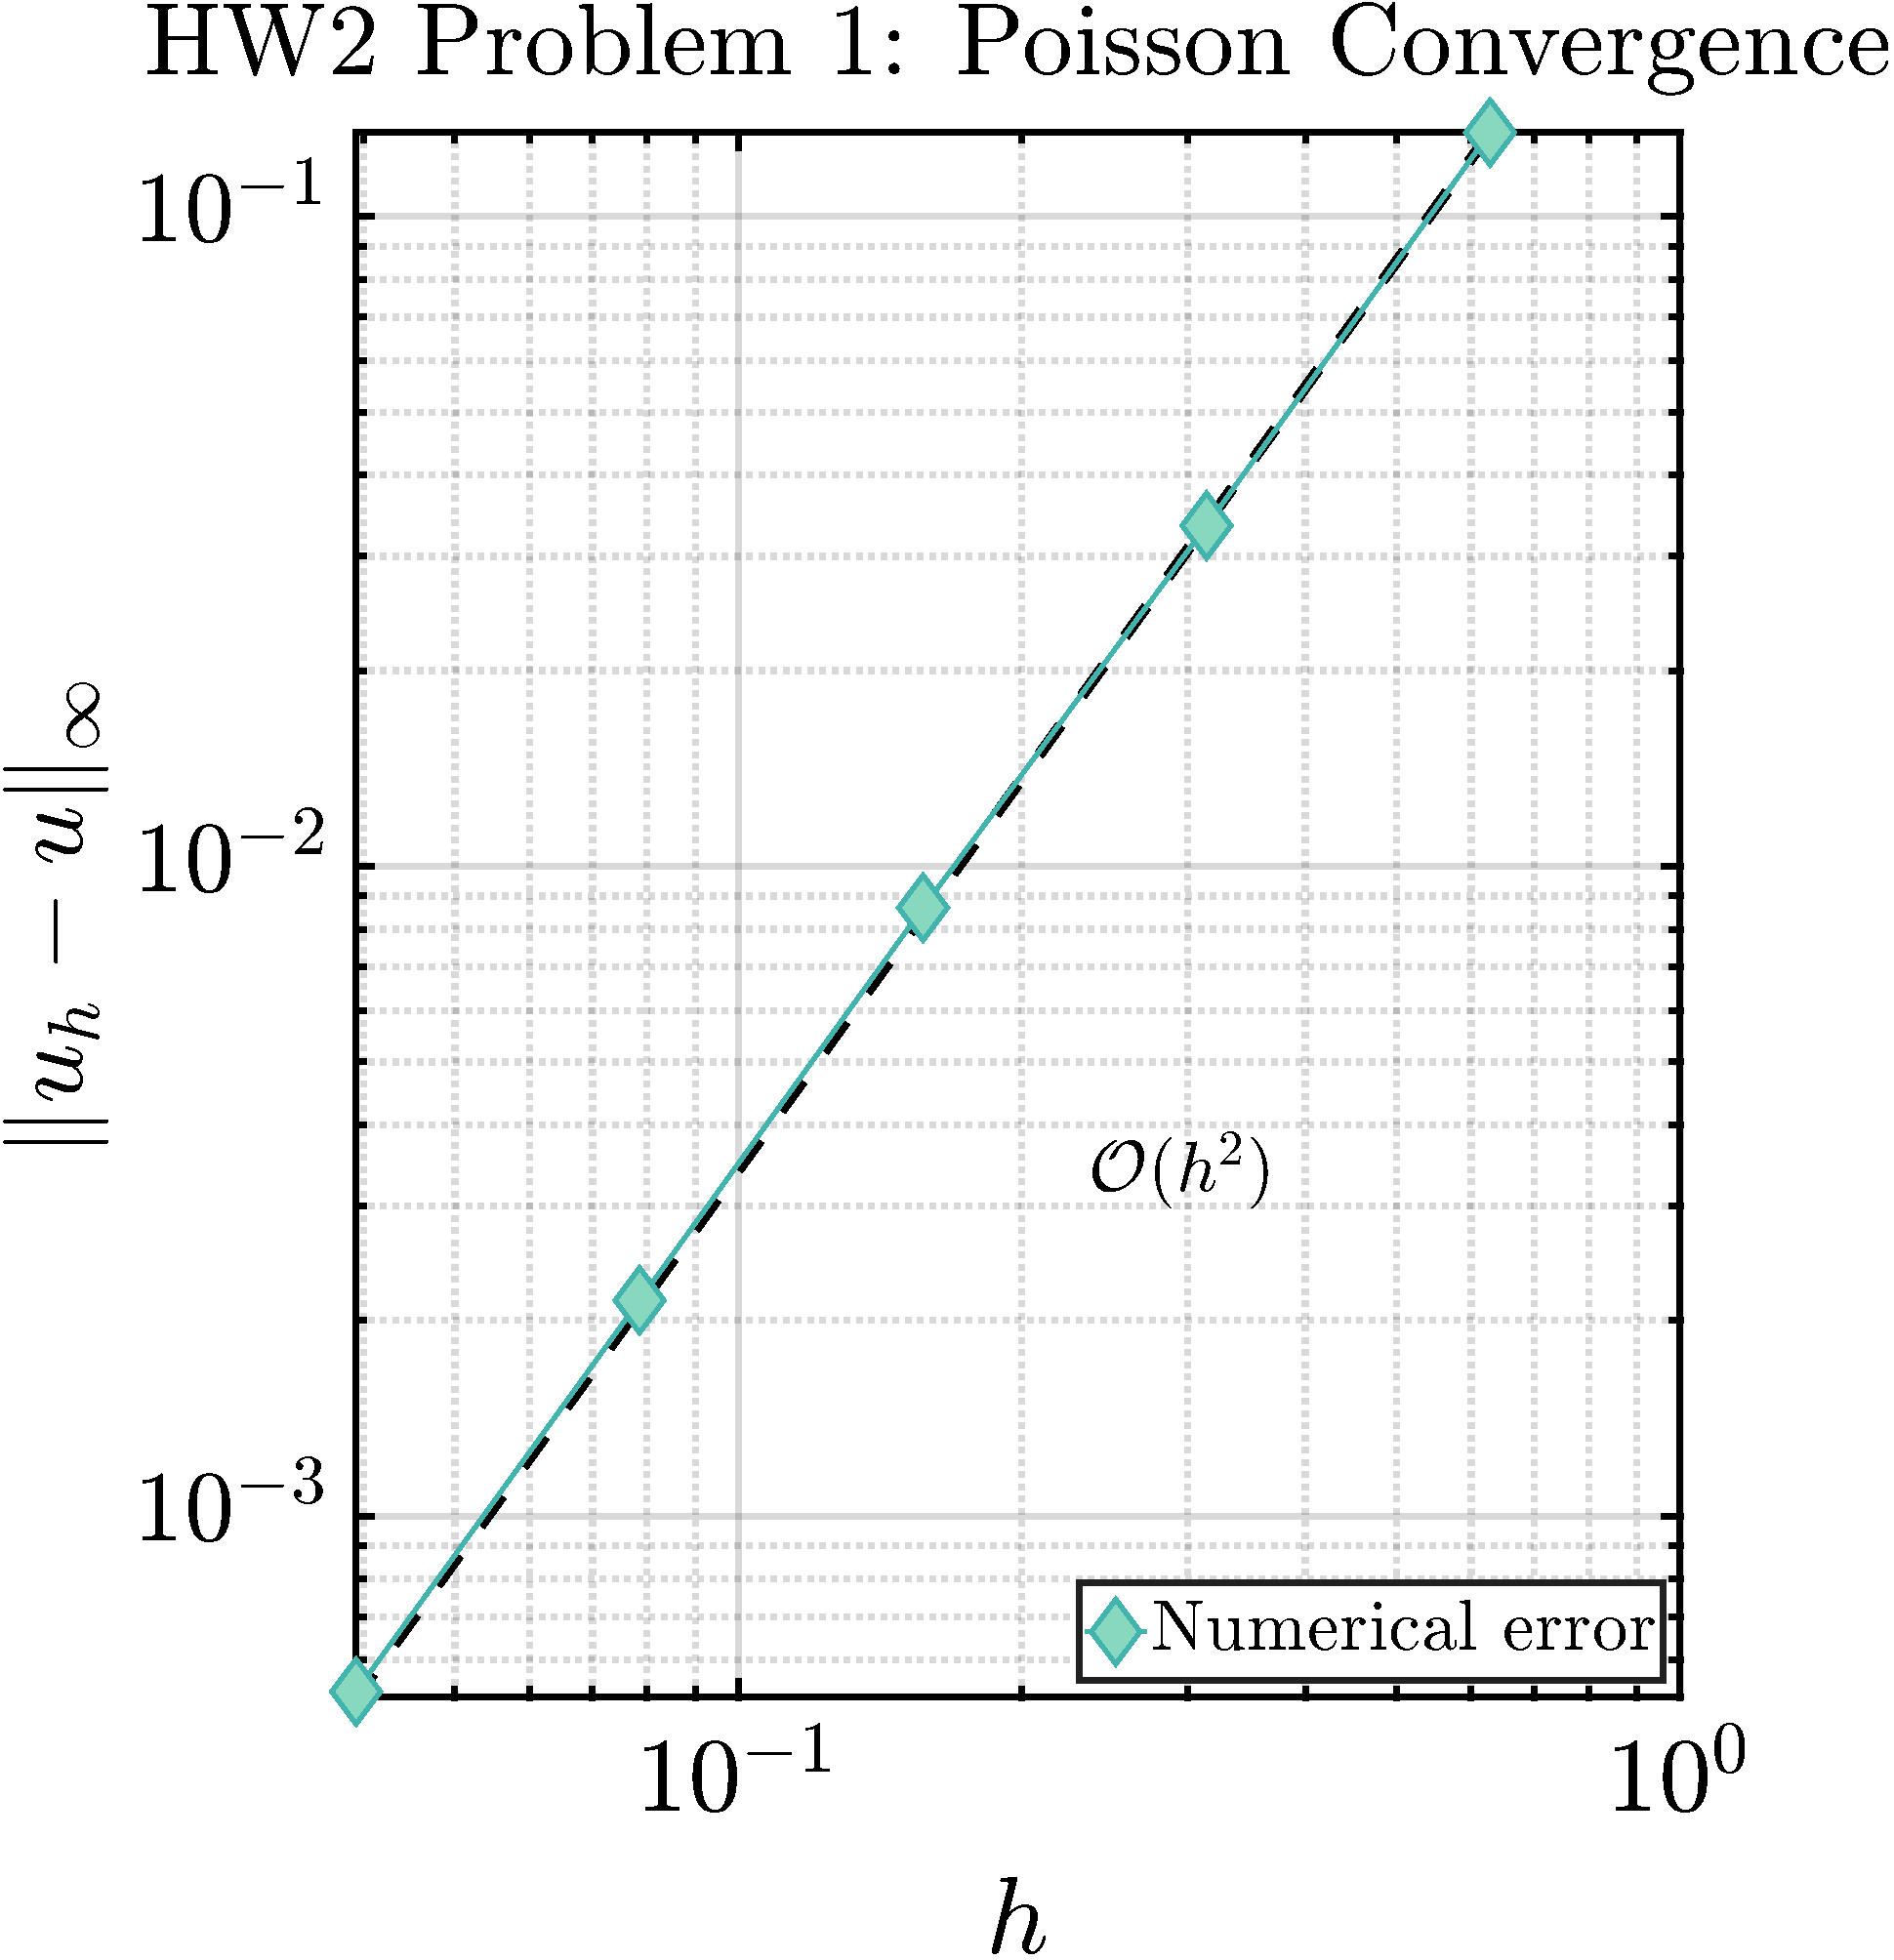
\includegraphics[width=0.40\linewidth]{poisson_hw2_problem1_convergence.pdf}
    \caption{Maximum absolute error $\norm{u_h-u}_\infty$ versus grid spacing
    $h$ on log-log axes with $\mathcal{O}(h^2)$ reference also pictured.}
    \label{fig:poisson-convergence}
  \end{figure}

Figure 1 showcases the approximate solution derived by the finite difference method as well as the exact solution. Figure 2 plots the $L^\infty $ error vs the grid spacing $h$. Plotted also is the reference $\mathcal{O}(h^2)$ slope, from which we can confirm that the error of this approximation is indeed proportional to the square of the grid size.
% --------------------------------------------------
\section{Poisson Equation with Immersed Boundary}
% --------------------------------------------------

We now look towards extending the solution above after having introduced a circular immersed boundary in the domain, given by:
\begin{align*}
  x_{\mathrm{IB}}=\pi+\cos\theta,\qquad
y_{\mathrm{IB}}=\pi+\sin\theta,
\quad \theta\in[0,2\pi].
\end{align*}

The Dirichlet condition is obtained from the above manufactured solution. We discretize the immersed boundary approximate a delta function using a 2d Gaussian to construct the spreading and interpolation operators. The resulting system is solved using the Matlab GMRES solver. The following are the results:

\begin{figure}[H]
    \centering
    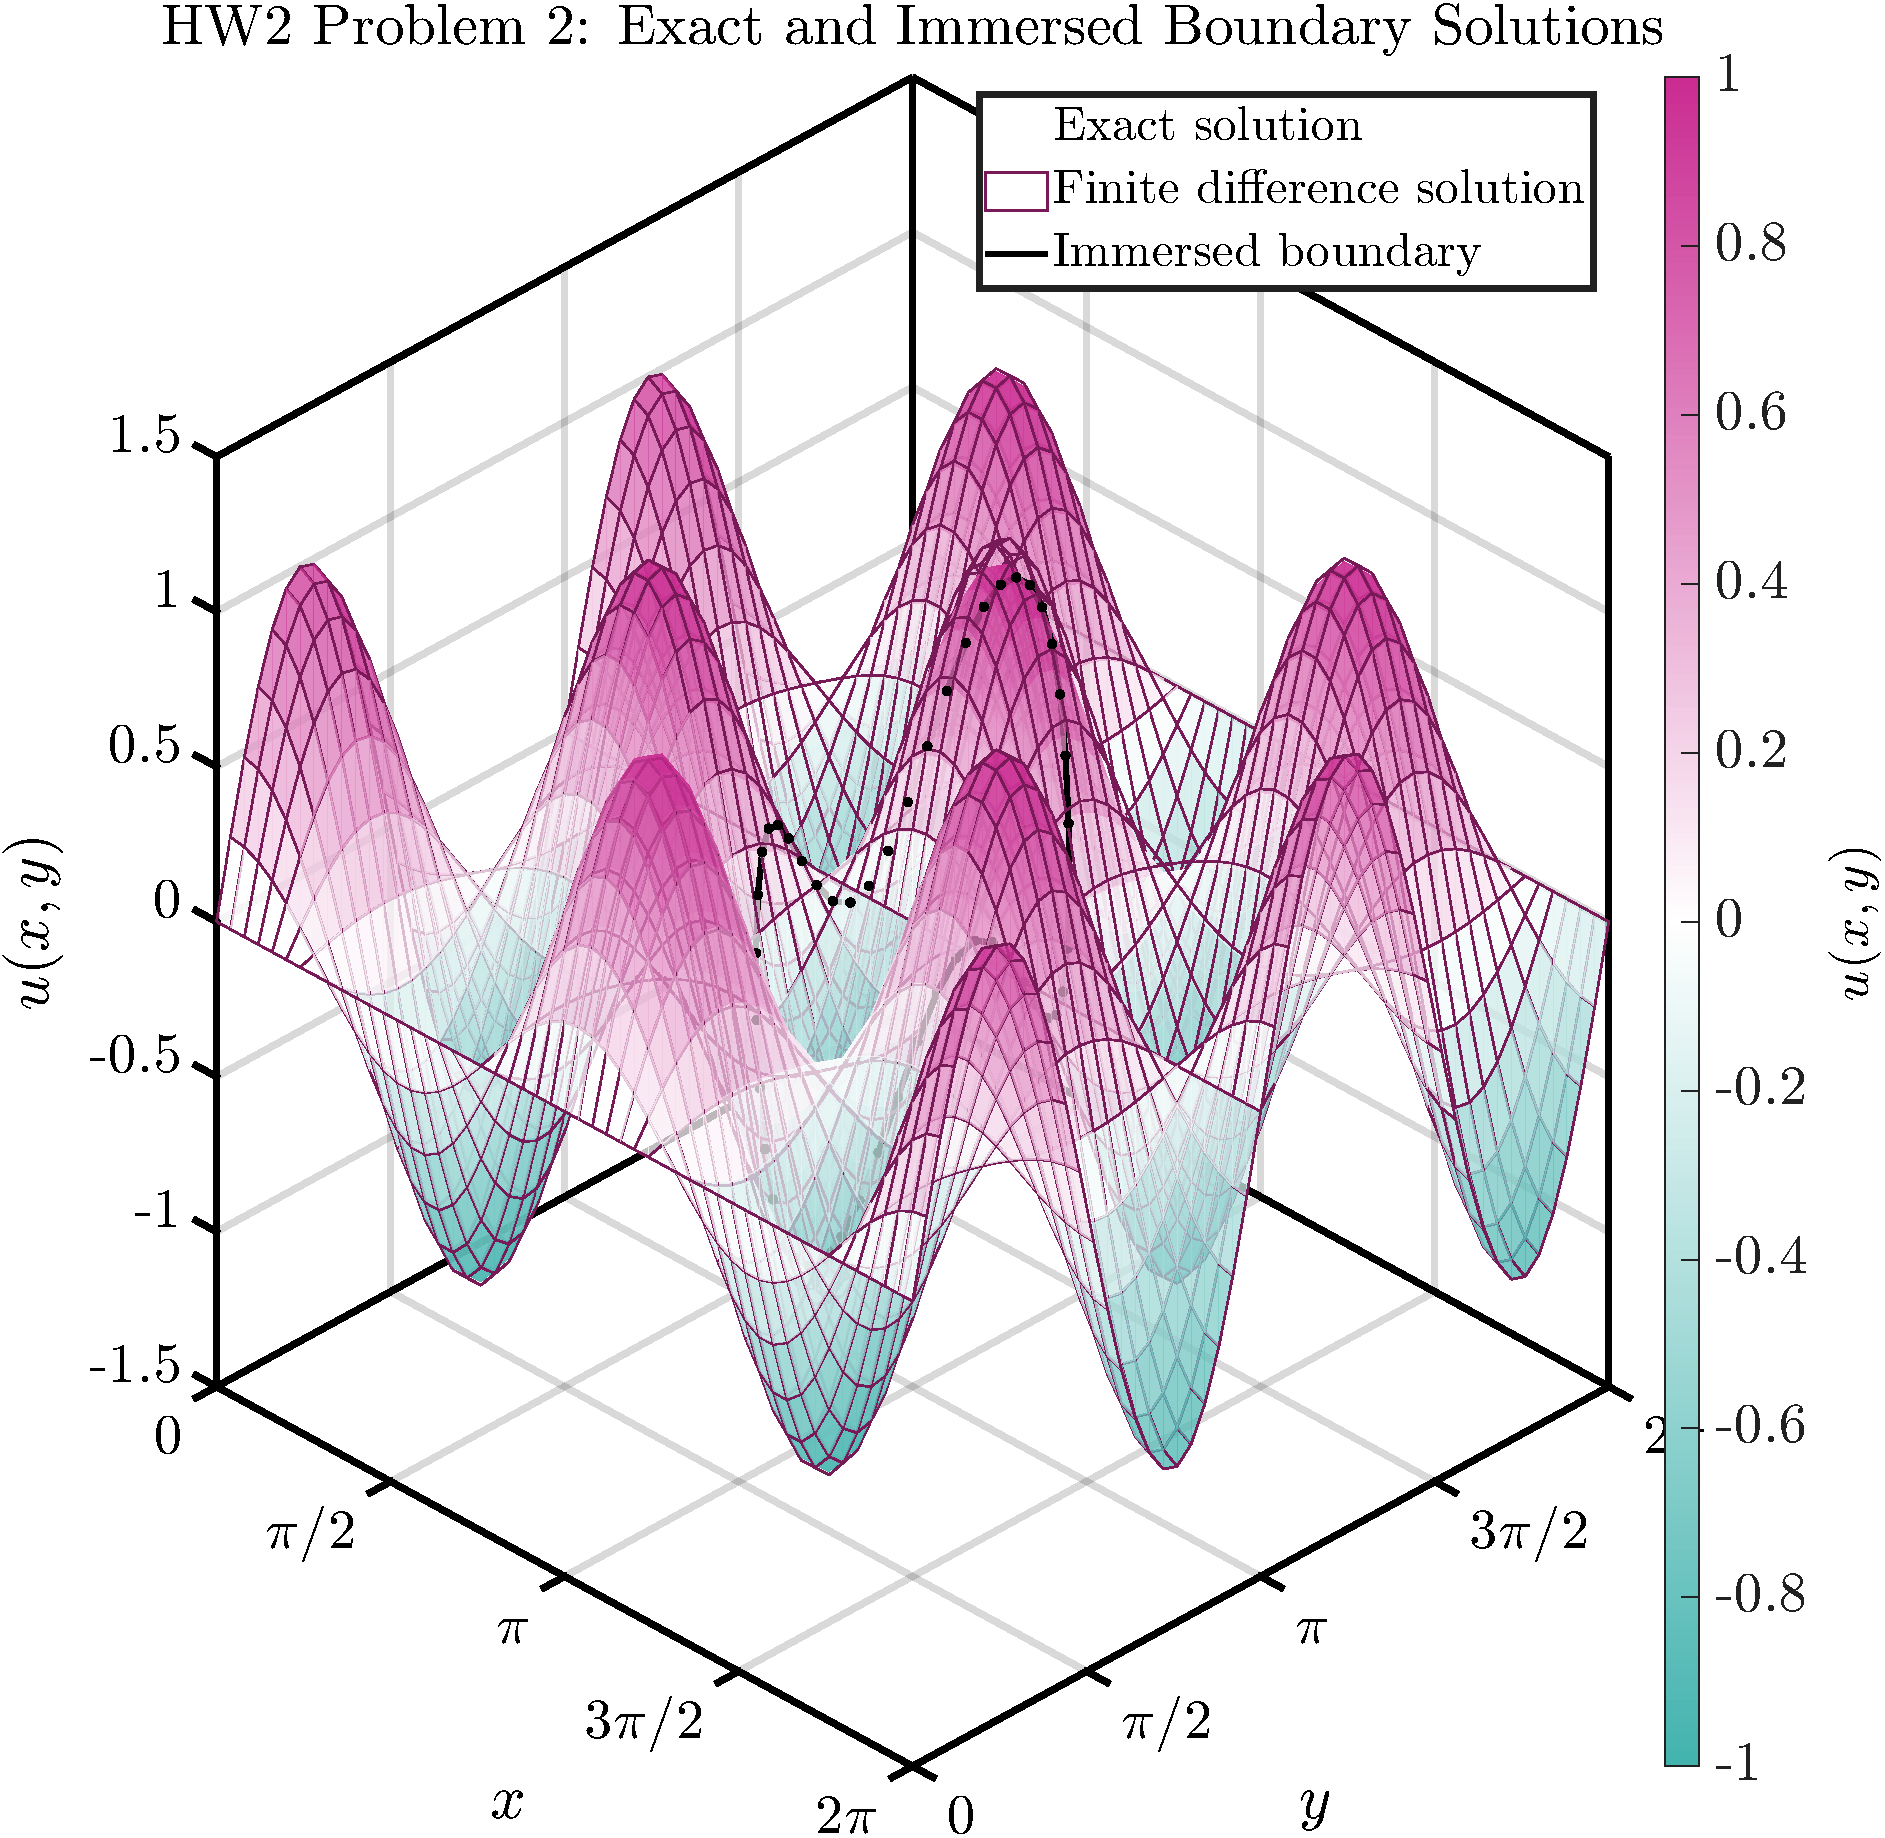
\includegraphics[width=0.55\linewidth]{poisson_hw2_problem2_solution.pdf}
    \caption{Exact solution with the finite-difference solution on
    $\Omega=(0,2\pi)^2$. The black curve with markers is the immersed
    boundary at the prescribed heights.}
    \label{fig:ib-solution}
\end{figure}

\begin{figure}[H]
    \centering
    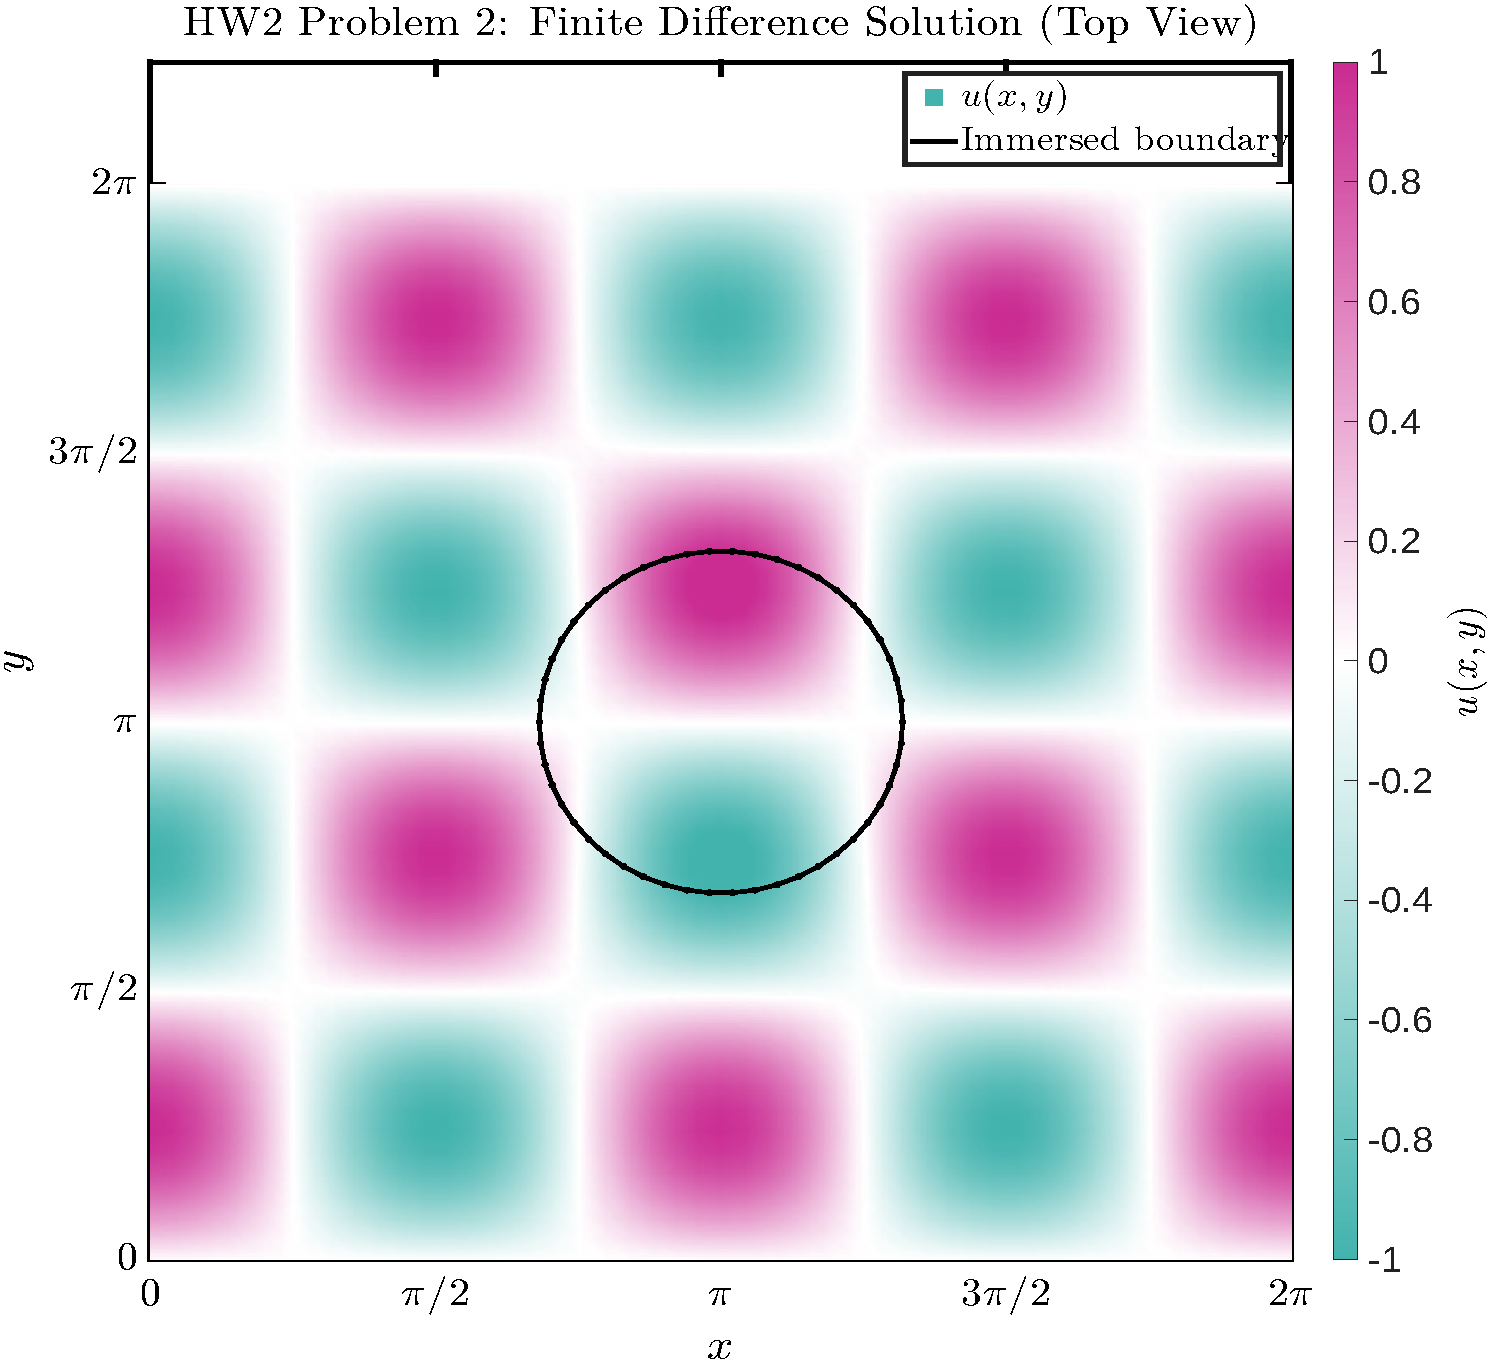
\includegraphics[width=0.55\linewidth]{poisson_hw2_problem2_top.pdf}
    \caption{Top view of the finite-difference solution. The black curve marks the immersed boundary
    with the $N_{\mathrm{IB}}$ marker locations.}
    \label{fig:ib-top}
  \end{figure}

As can be observed, the numerical solution does closely match the manufactured solution, even near the immersed boundary. Therefore, we see that the immersed boundary constraint is being enforced without a significant consequence to the expected solution

\begin{figure}[H]
    \centering
    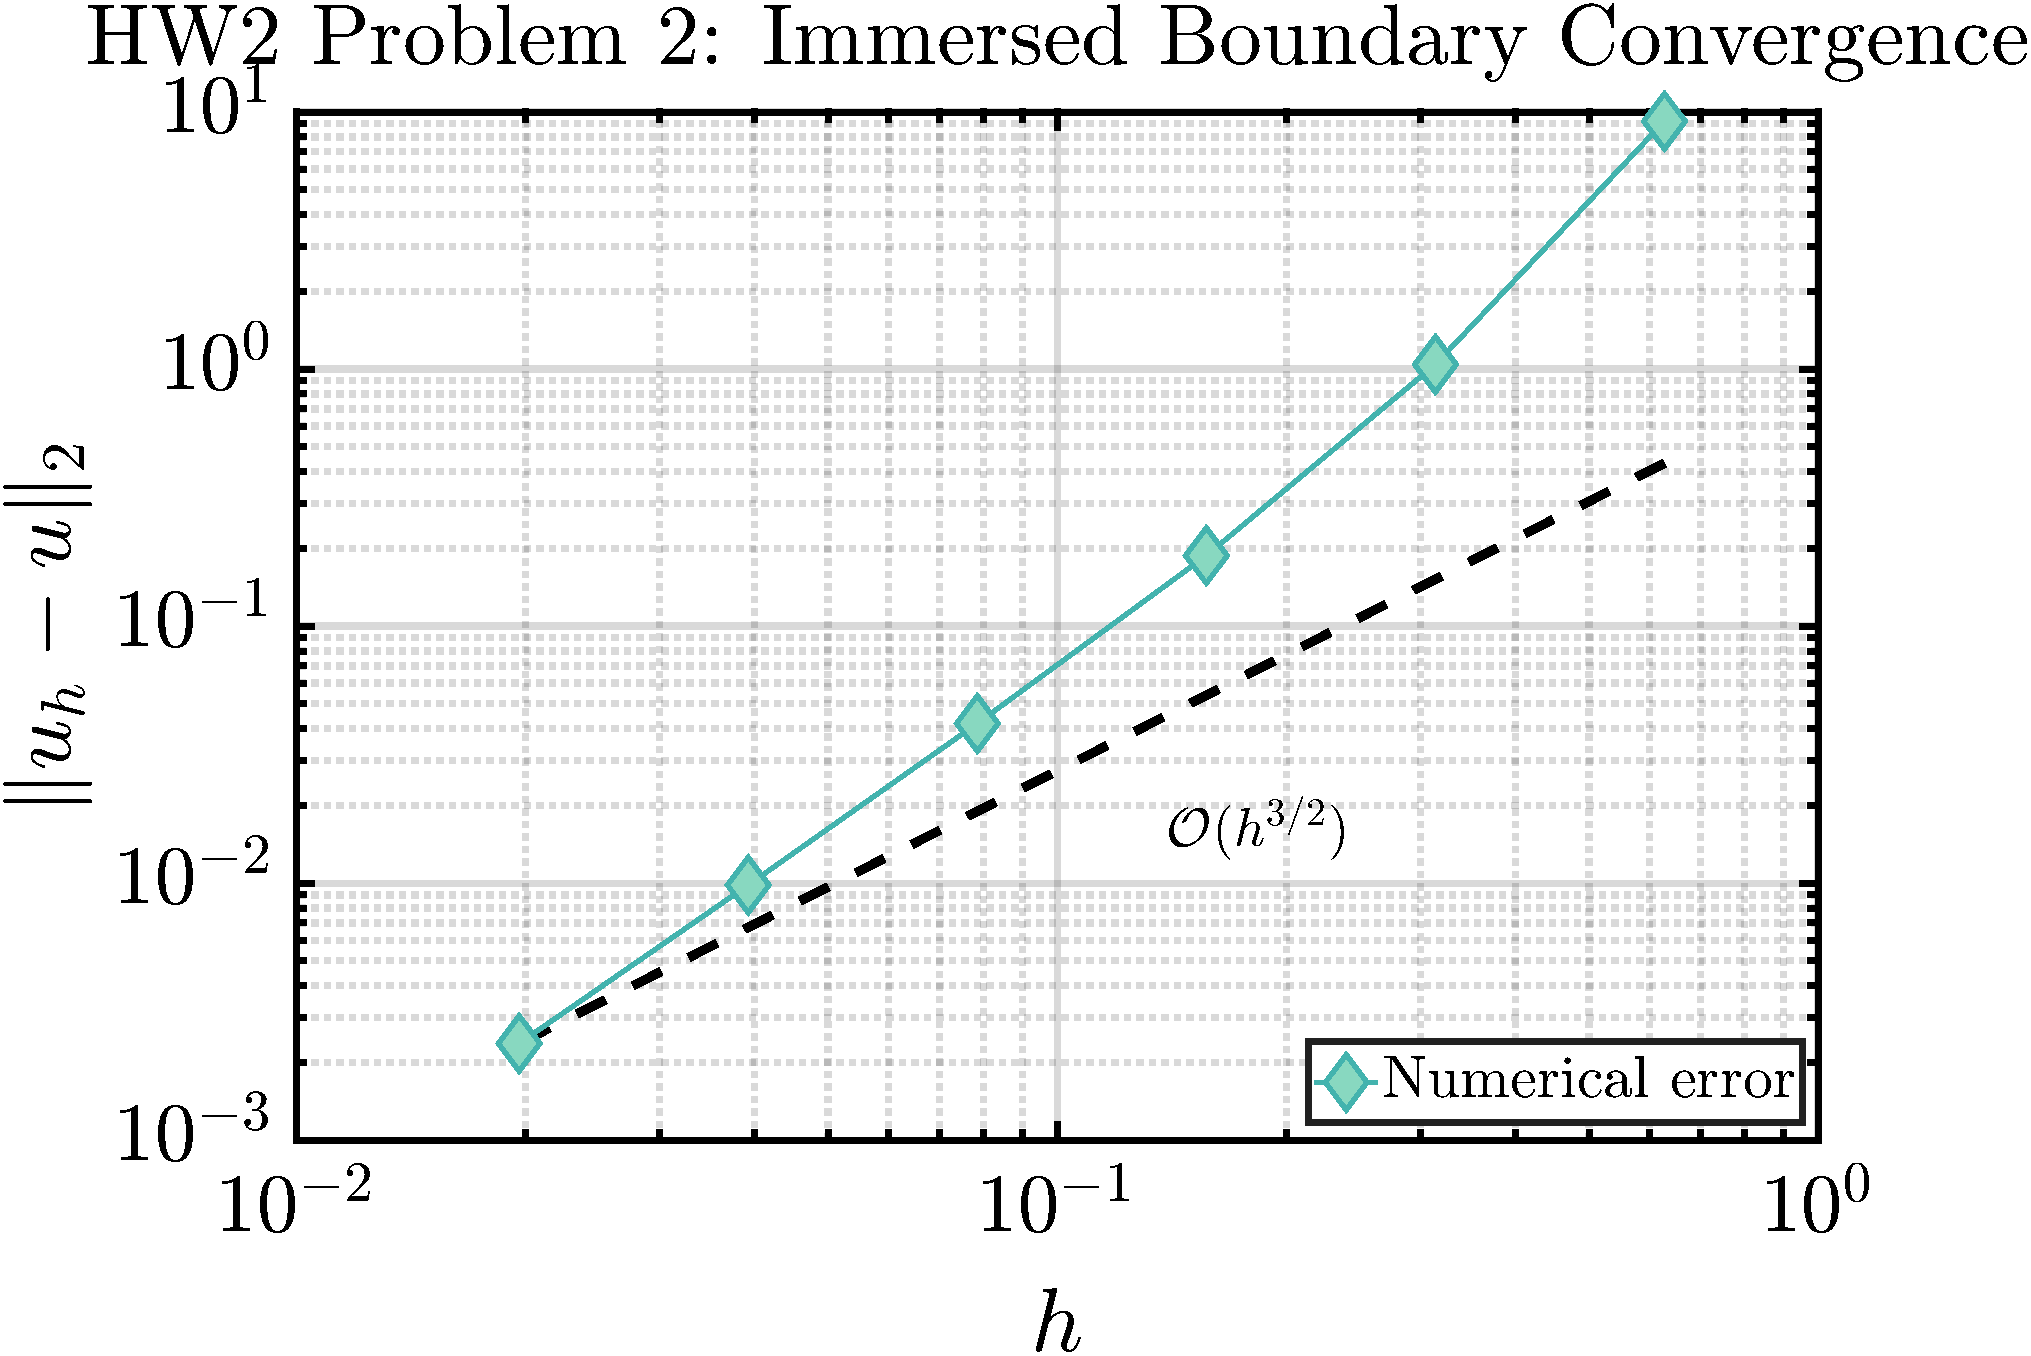
\includegraphics[width=0.50\linewidth]{poisson_hw2_problem2_convergence.pdf}
    \caption{Discrete $L^2$ error $\norm{u_h-u}_{2}$ versus grid spacing $h$
    on log-log axes.}
    \label{fig:ib-convergence}
  \end{figure}

  We do see that the error decreases at every refinement. The convergence rate is higher than originally expected, but at finer gird resolutions, we see that the error curve approaches the slope of the $\mathcal{O}(h^{3/2})$ reference line.


% --------------------------------------------------
\section{Almost Minimal Surface}
% --------------------------------------------------
We can now adjust the boundary conditions to find a solution to the almost minimal surface problem. Imposing homogeneous Dirichlet boundary conditions and setting removing the forcing yields the following solution:

\begin{figure}[H]
    \centering
    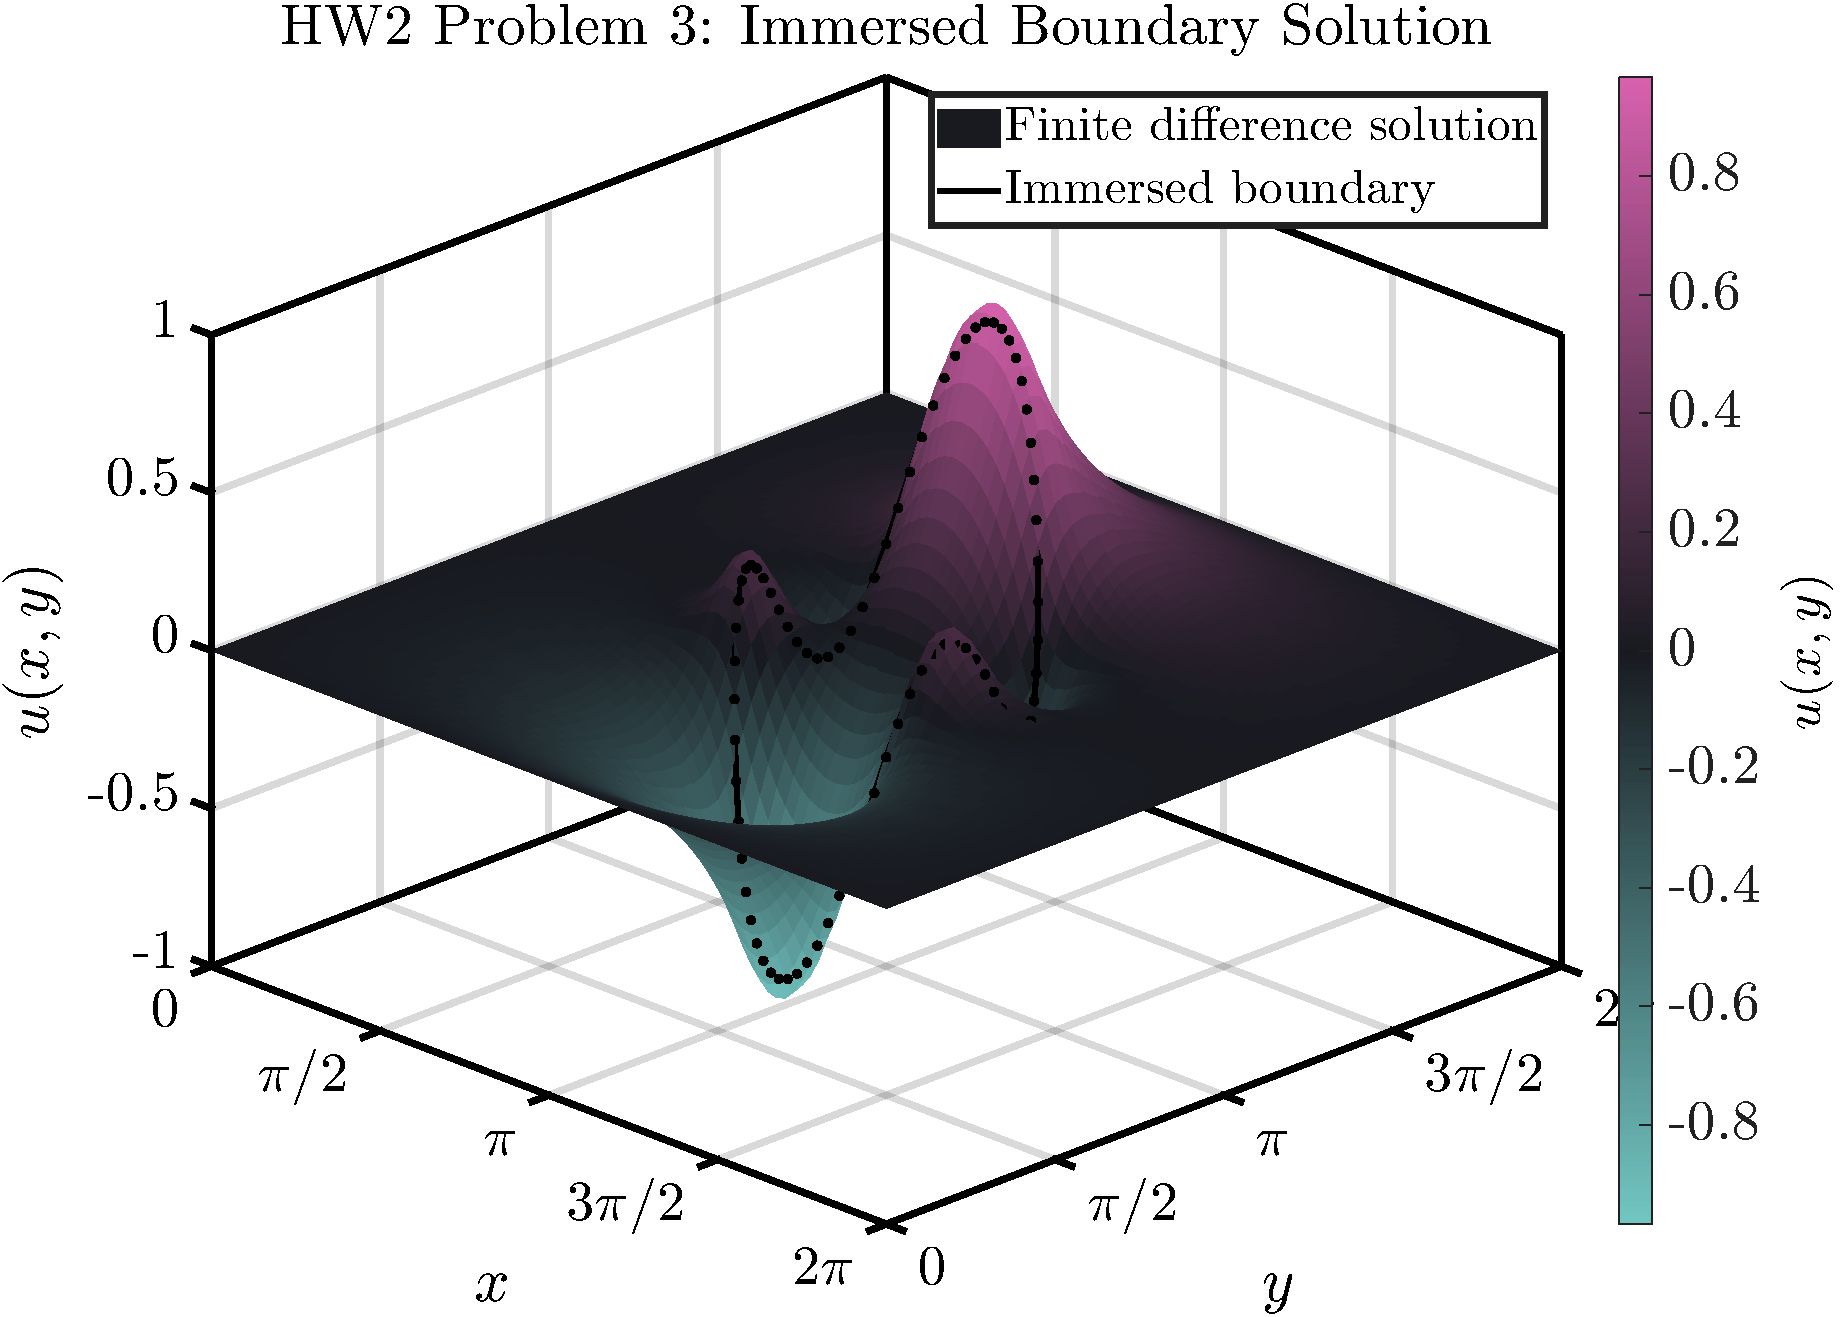
\includegraphics[width=0.55\linewidth]{poisson_hw2_problem3_solution.pdf}
    \caption{Numerical solution $u$ of $\lap u = S^{\mathrm{IB}}(q)$ with
    $u=0$ on $\partial\Omega$ and $u = \cos 2x \sin 2y$ prescribed on the
    immersed boundary}
    \label{fig:minimal-surface}
\end{figure}


% --------------------------------------------------
\section{Additional Experiment: Multiple Shapes}
% --------------------------------------------------

We now look towards modifying the immersed boundary method developed in the preceding sections to implement multiple immersed boundaries in the domain. We introduce two circular boundaries of radius $r= 0.65$ cantered at $(\pi -1.25,\pi )$ and $(\pi +1.25, \pi )$. We prescribed a value of $u = 1$ for the left circle, and $u=-1$ for the right circle.

Thankfully, we can preserved much of the implementation from the previous section, except that we now combine the two immersed boundary points into one system, reconstruct the spreading and interpolation operators, and use GMRES to solve the saddle system:

\begin{figure}[H]
    \centering
    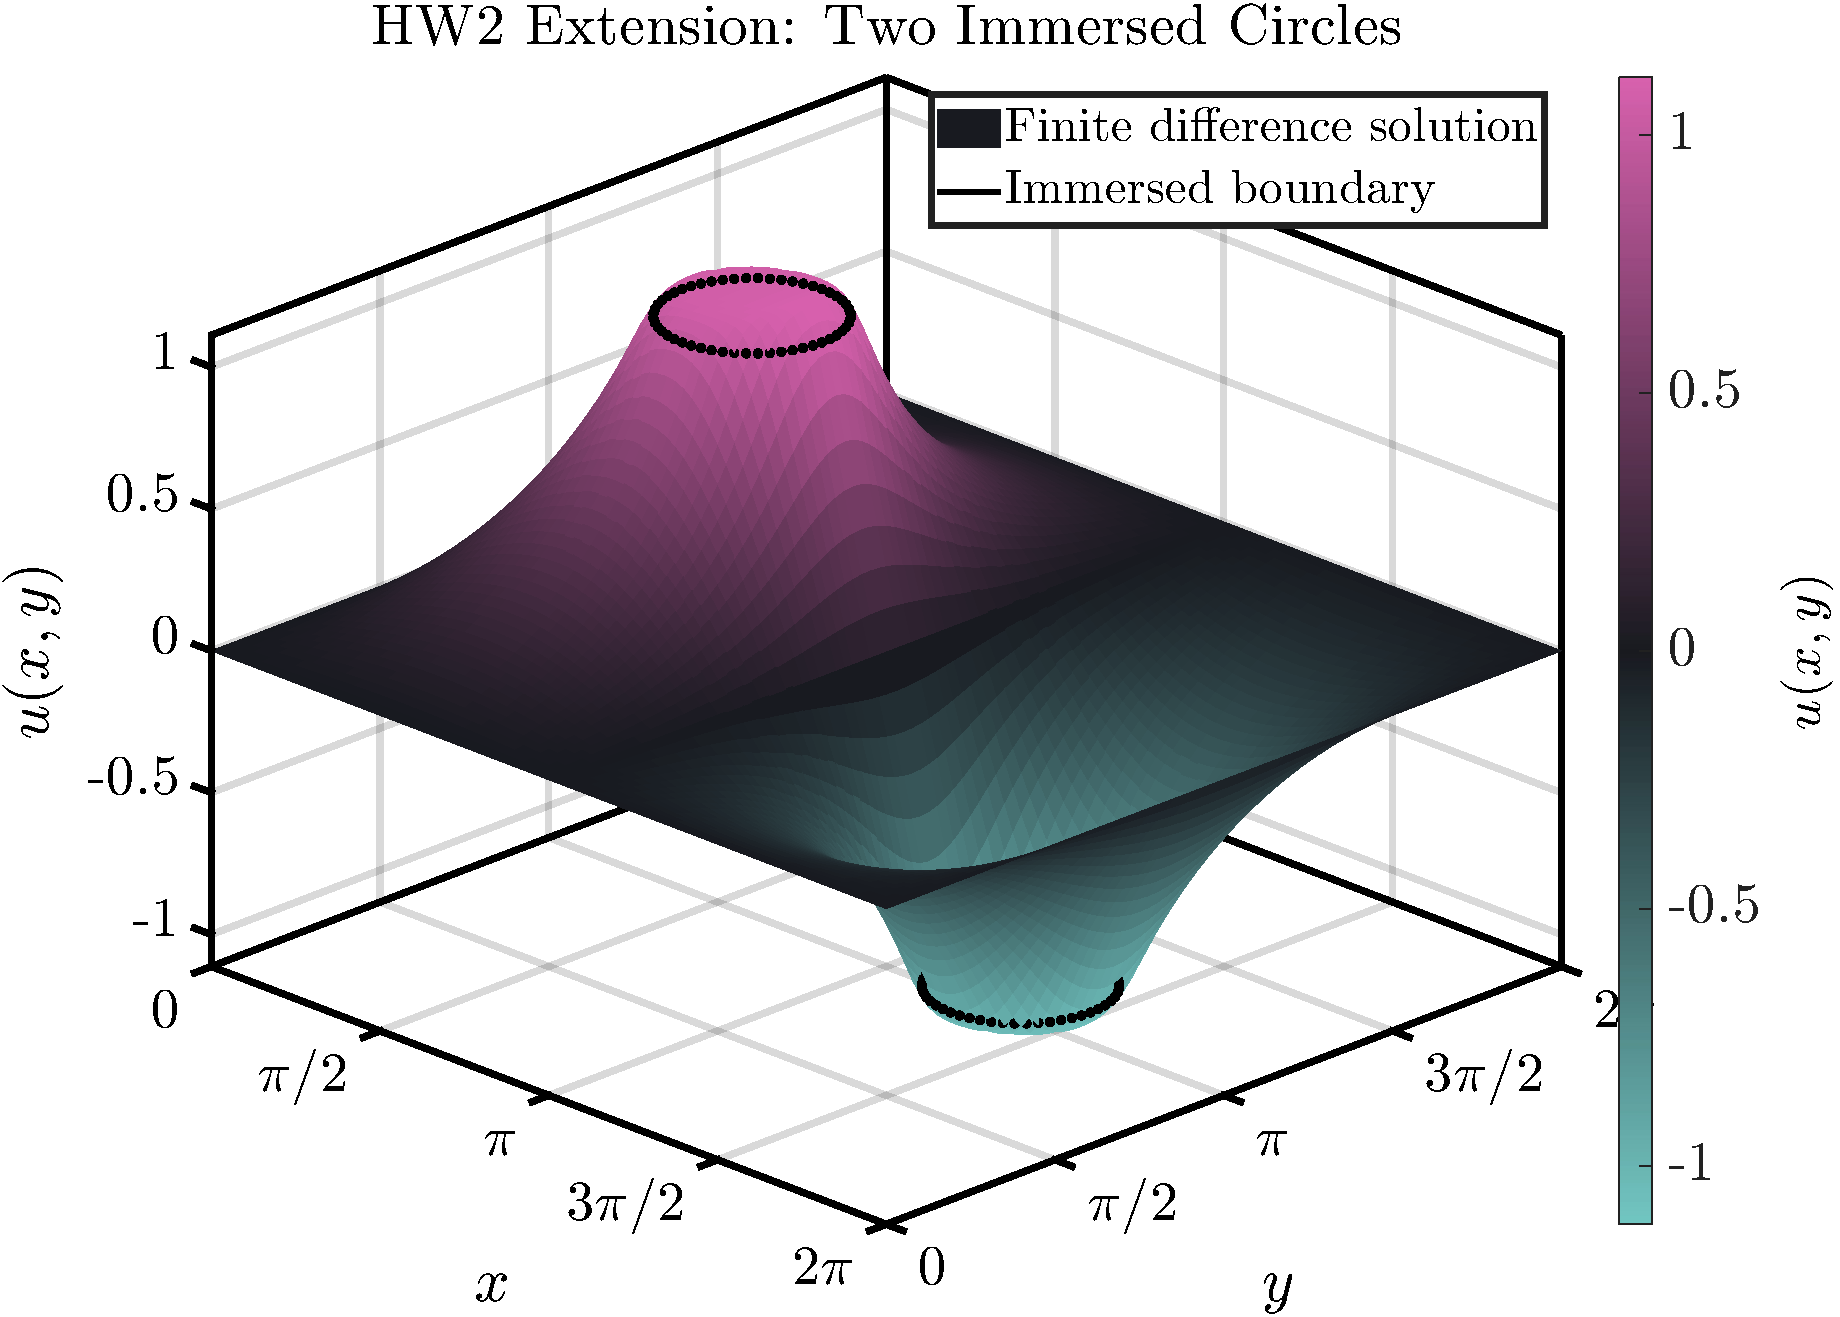
\includegraphics[width=0.55\linewidth]{poisson_hw2_two_circles_solution.pdf}
    \caption{Numerical solution $u$ of $\lap u = S^{\mathrm{IB}}(q)$ with
    $u=0$ on $\partial\Omega$ and two circular immersed boundaries with $u=1$ and $u=-1$}
    \label{fig:two-circles}
\end{figure}

The solution has positive and negative regions corresponding to the values prescribed on the two immersed boundaries, as well as approach 0 near the outer boundary. The behavior of the solution indeed demonstrates how several immersed boundaries can be inserted into the domain of the Poisson equation without substantially altering the underlying grid.

% --------------------------------------------------
\section{AI Use Disclosure}
% --------------------------------------------------
AI was used to plot all graphs in the manner dictated by conventions outlined in the textbook for the course, as well as to facilitate learning about spreading and interpolation operator theory (ultimately wasn't too important). It was also used to provide examples of functioning code from which to learn, since the code and methods necessary to complete the assignment were complex relative to my understanding. It was also helpful at summarizing the ideas in Peskin's Immersed Boundary Methods paper/textbook. Opencode agent running GLM 5.3 Flash was used to generate the README.md.


\end{document}
